\section{Log Replication} % (fold)
\label{sec:log_replication}

In this section we will describe how Raft handles log replication, discuss some of the design decisions we have taken within Raft and describe the challenges with the implementation.

\subsection{Log Replication in Raft} % (fold)
\label{sub:log_replication_in_raft}

The general purpose of the log replication feature in a consens algorithm and in Raft is to keep a log history of commands applied to the state machine in order to compare integrity between servers.

Log entries are appended to the log when a client requests a given command to be applied. The flow of receiving the request from the client, commiting the command to the log and responding the client is illustrated in figure~\ref{fig:log_replication_example}. In overall the steps of committing a command in Raft can be written as:

\begin{enumerate}
  \item Client sends request to the leader with command
  \item Leader appends command to own log
  \item Leader replicates log to followers in parallel
  \item When the command is replicated and commited to a majority of the servers in the cluster, the leader will respond positively to the client and apply the command to the state machine. \label{enum:client_request_final}

\end{enumerate}

\begin{figure}[ht!]
  \centering
  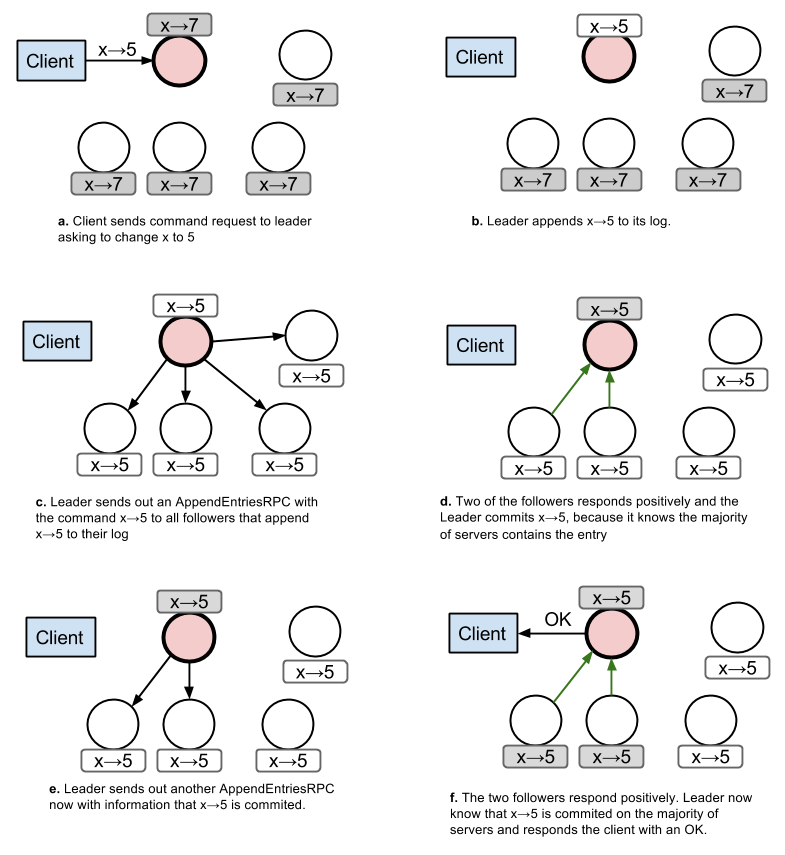
\includegraphics[width=0.7\textwidth]{figures/log-replication-example.png}
  \caption{An illustration of how the leader succesfully apply a command from the client. At first \emph{(a)} the client requests the leader to apply the command x$\rightarrow$5 to the state machine, then \emph{(b)} the applies the command to its own log and \emph{(c)} replicates it to the followers. \emph{(d)} The followers respond positively if the command is applied to their log and the leader commits the entry from the client, when a majority of the servers have appended the log. \emph{(e)} The followers will receive information that the entry is commited and \emph{(f)} when the leader knows that a majority of the servers have applied the command, it will respond to the client positively and append it to the state machine}
  \label{fig:log_replication_example}
\end{figure}

% Maybe do not include this headerline
\subsubsection{AppendEntries RPC/Heartbeat} % (fold)
\label{ssub:appendentries_rpc_heartbeat}

The log replication mechanism explained in these steps are in Raft the same heartbeat mechanism used for claiming leadership as explained in section~\ref{sec:leader_election}. The hearbeat/log replication request is a Remote Procedure Call (RPC) called \emph{AppendEntries RPC}. The leader invokes the RPC with information for the follower duplicate the leaders log and be in consensus. The follower then responds the leader with success if it is fully replicated or else failure.

% subsubsection appendentries_rpc_heartbeat (end)

% Maybe do not include this headerline
\subsubsection{Commiting Log Entry} % (fold)
\label{ssub:commiting_log_entry}

The first time a server receives an AppendEntries RPC it will just append it to the log. A log entry is committed by the leader when the leader knows that a majority of the servers have appended the given log entry to their log. The log entry is then commited on a follower, when the leader sends out information (through \emph{AppendEntries RPC}) that the index of a given log entry is commited. The log entry is safe to apply to the state machine, when a majority of the servers have commited the entry.

% subsubsection commiting_log_entry (end)

\subsection{Handling Log Inconsistency} % (fold)
\label{sub:handling_log_inconsistency}

The scenario explained this far is the sucessful one, but in distributed systems failures such as network partitions and single server crashes are not rare and should be handled. Raft have behaviour for handling different kind of log inconstencies, which compared to the true log of the leader can be:

\begin{enumerate}
  \item A follower is missing entries
  \item A follower has extra entries
  \item A follower is both missin entries and has extra entries
\end{enumerate}

All situations of inconcistencies are handled by forcing the followers to duplicate the leaders log. The first situation is handled through the AppendEntries RPC by finding the largest common commited index and replicate the missing entries from the leader. The second scenario is handled by finding the largest common commited index and delete all entries following. Thereafter the situation is as the first and handled so. The last scenario is handled as the second.

% subsection handling_log_inconsistency (end)

\subsection{Implementation} % (fold)
\label{sub:log_replication_implementation}

The log and heartbeat are two implementation specific parts of the Raft algorithm that is not described in implementation details.

Normally the log should be persistent meaning that it should be persisted to disk such that a failure would not result in data loss. But since the implementation in this project is only for visualization, persistency is not implemented. The log is implemented as an object \verb$Log$ that works as an abstraction on top of a simple array containing the entries. For a programmer this abstraction is important since Raft is documented and specified as being a 1-indexed system, where most databases and arrays in various programming languages are 0-indexed.



% Components
%   - The Log (store in array, abstracts the 1-indexing in Raft)
%   - LeaderState (the state the leader keeps about the followers)
%   - The Heartbeat ()

% subsection implementation (end)

% section log_replication (end)
